\documentclass[../thesis.tex]{subfiles}
\begin{document}

\chapter{parametric study}
\label{chp: para_stud}
Within the parametric study the three different reactor geometries are simulated under different flow conditions. These different conditions, as shown in \autoref{tab: cases}, lead to different front shapes. Two of these front shapes can be seen in \autoref{fig: shape_examp}.

\begin{figure}[htb]
	\centering
	\subfloat[\centering front shape for h0.6mm Pe2050 Sc12000]{{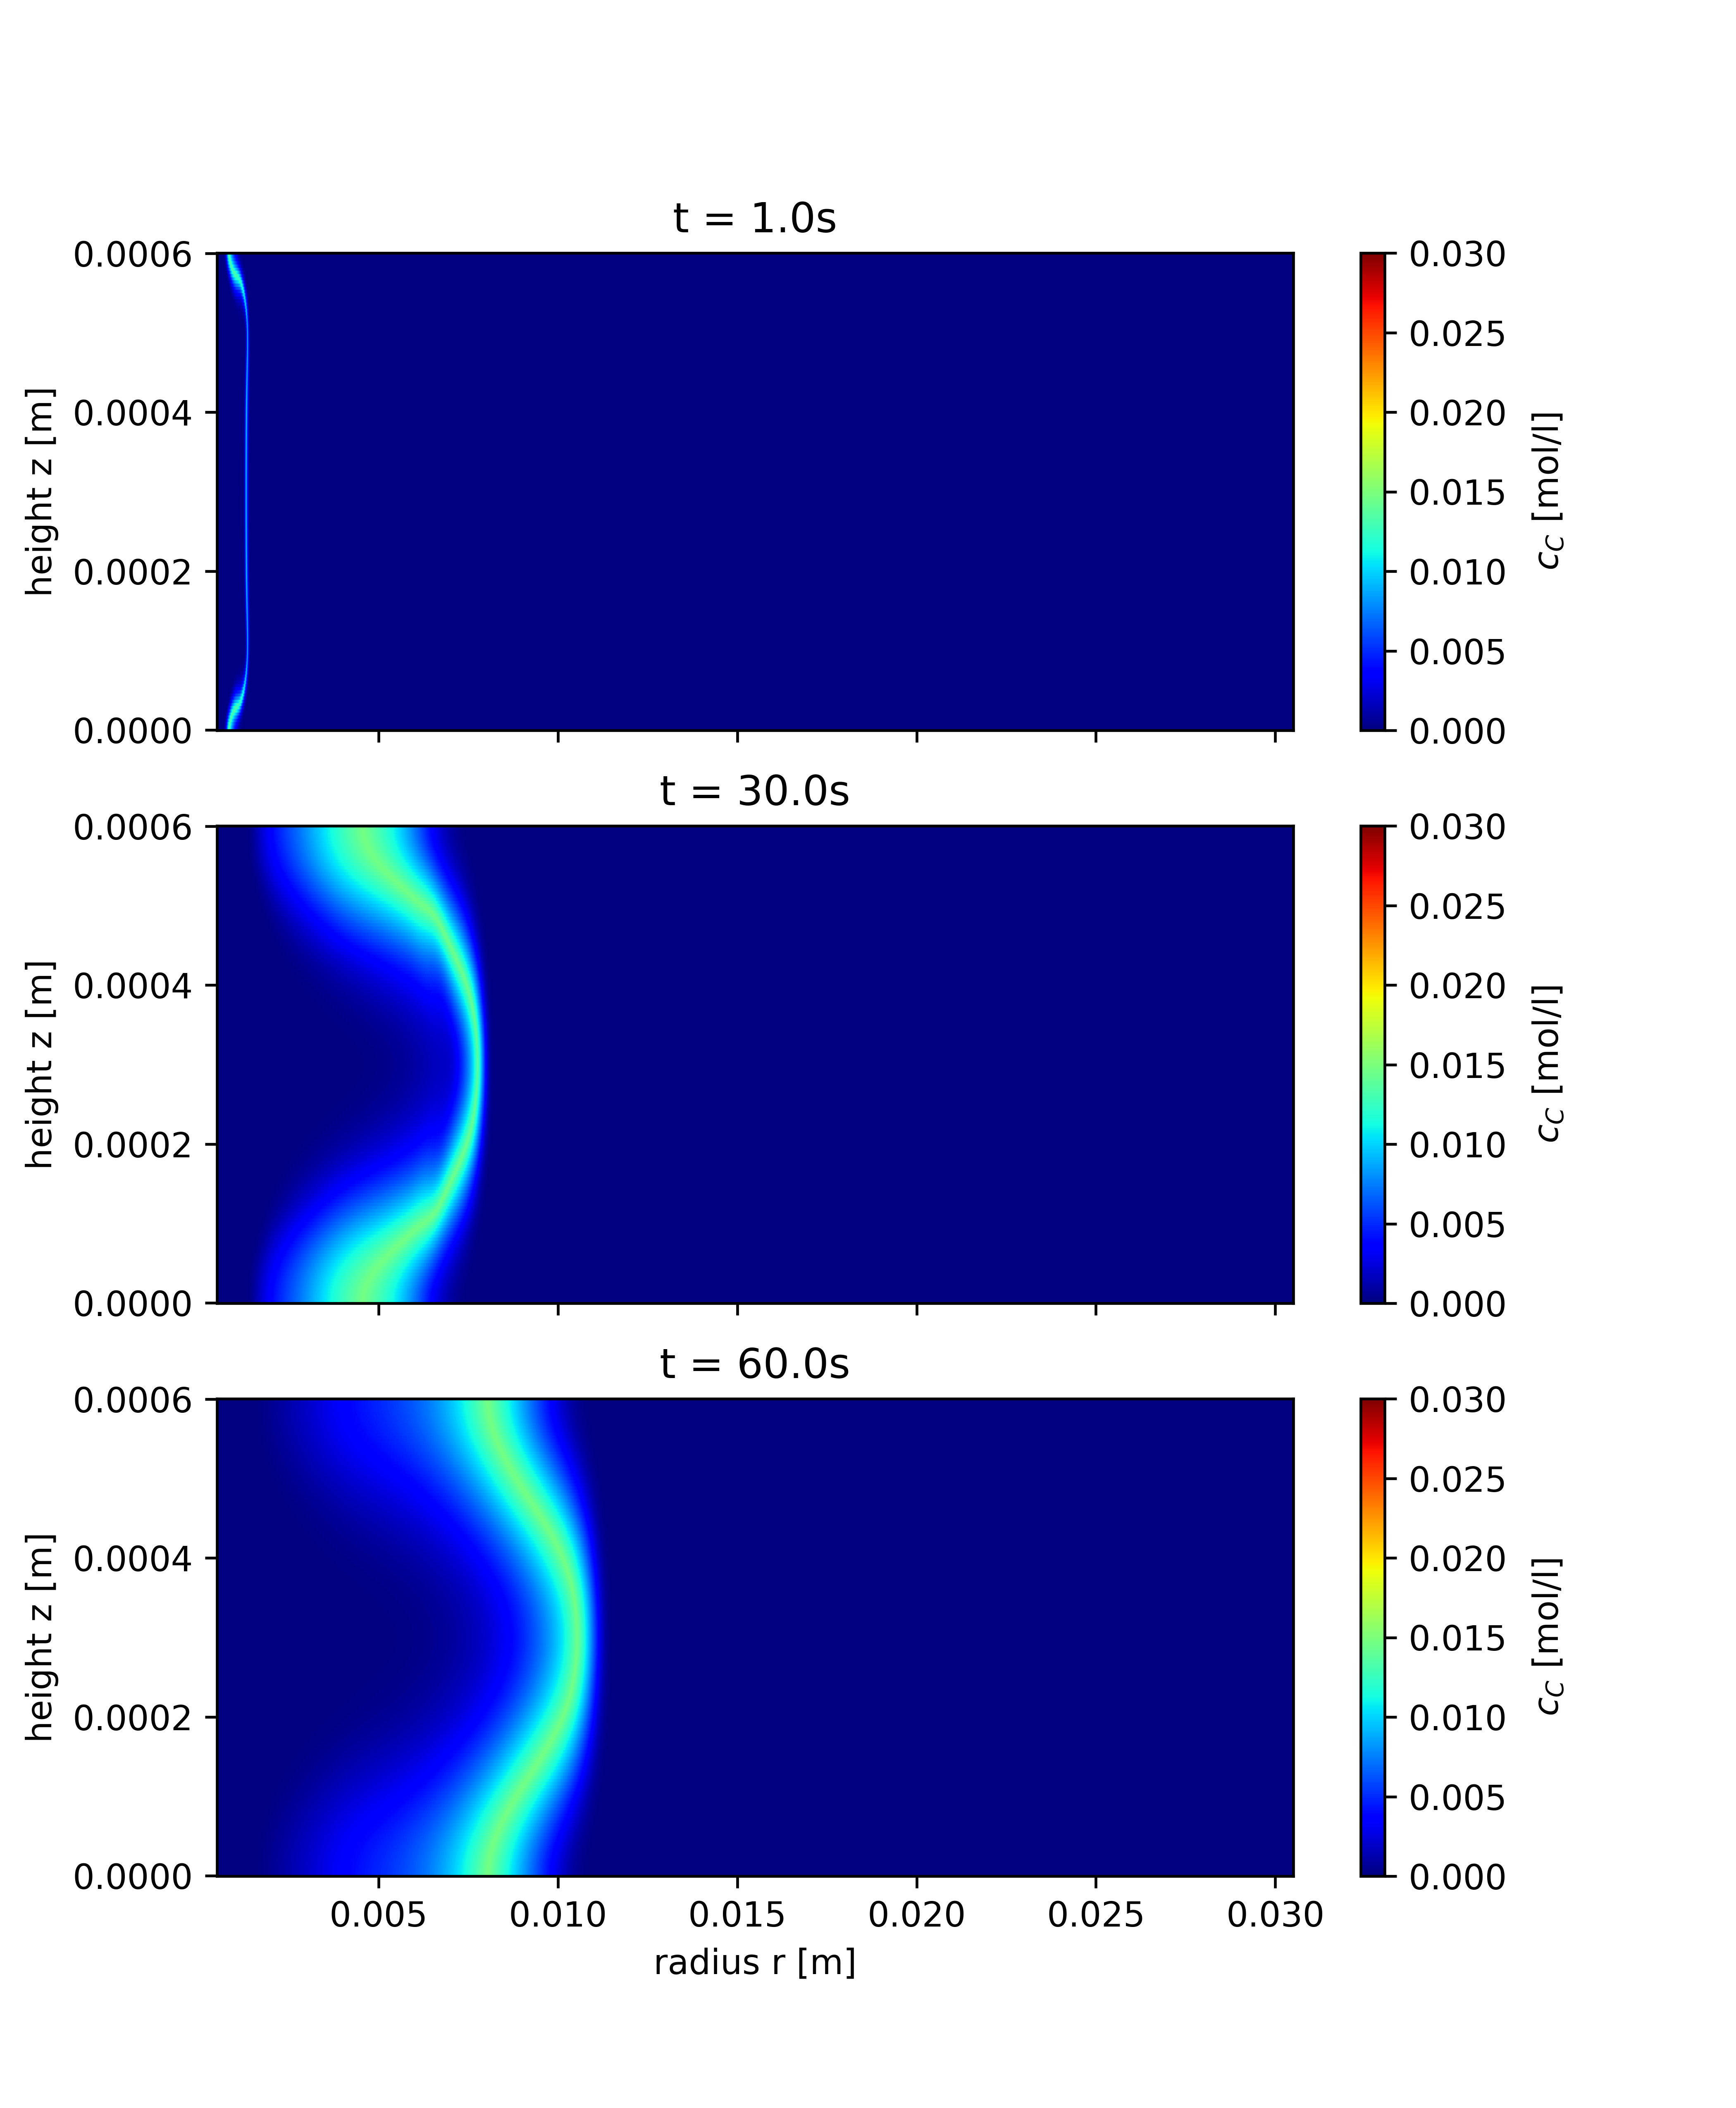
\includegraphics[angle=90, scale=0.55]{front_shape1} }}%
	\qquad
	\subfloat[\centering front shape for h0.2mm Pe2050 Sc2430]{{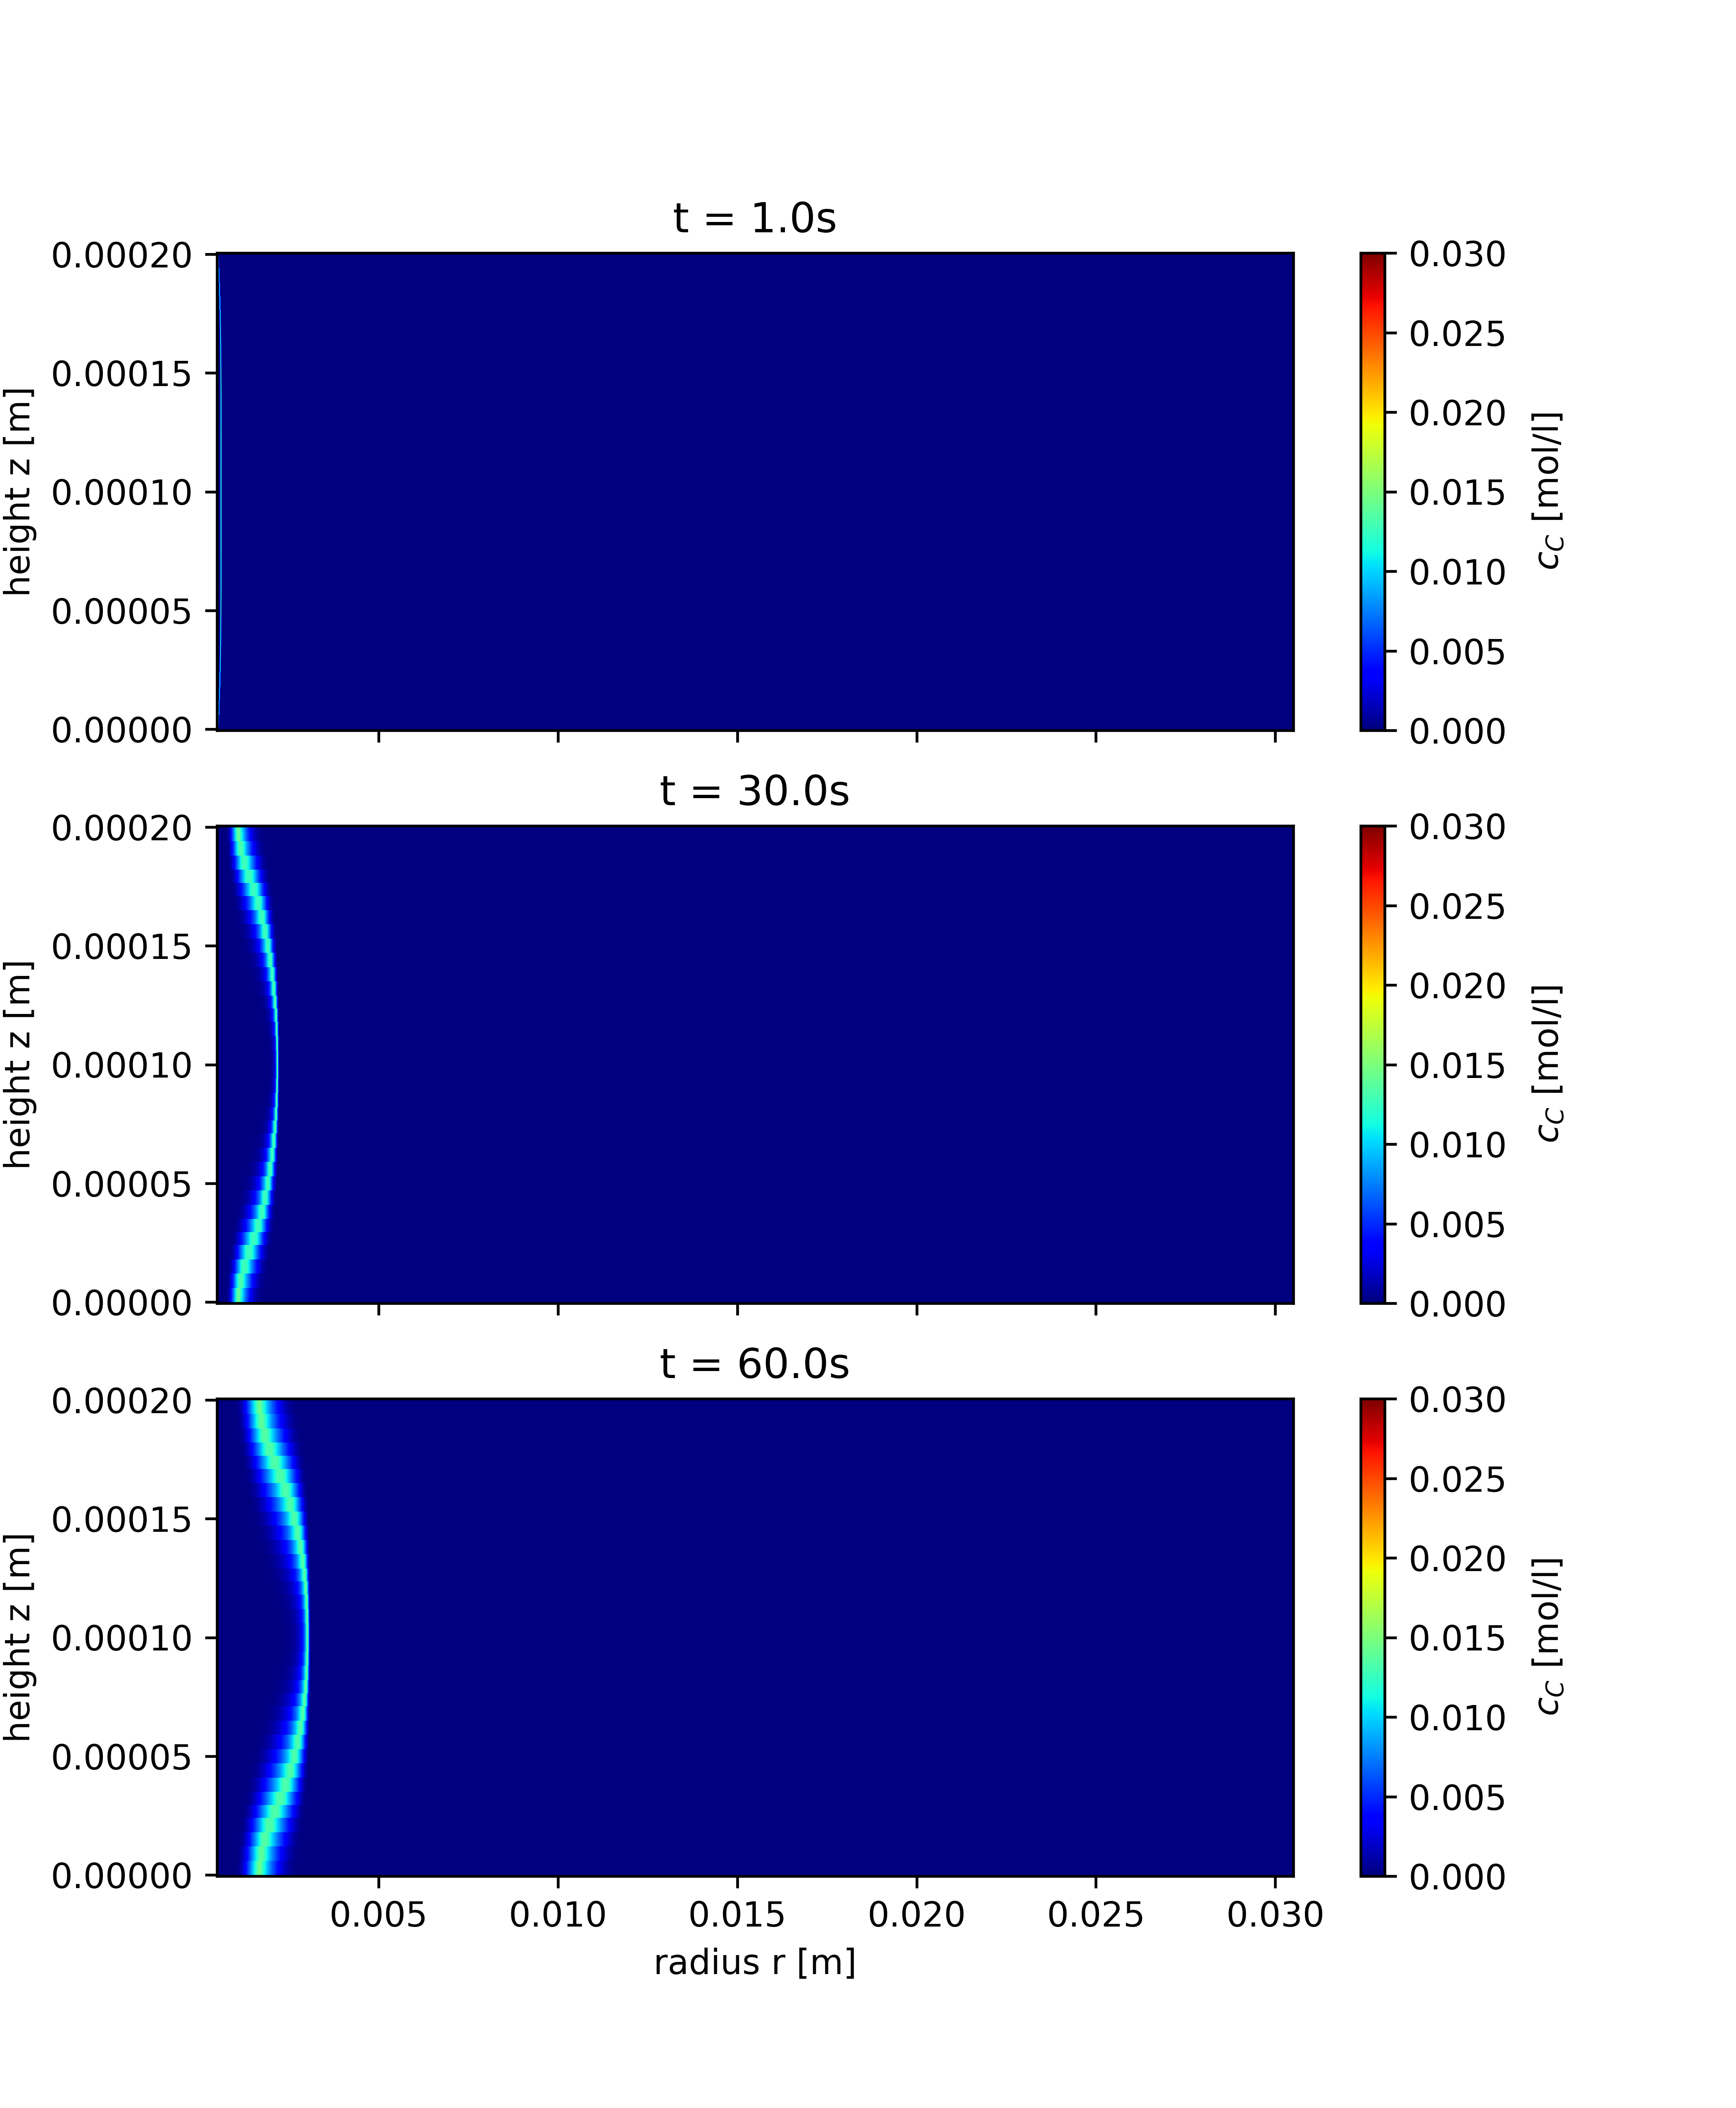
\includegraphics[angle=90, scale=0.55]{front_shape2} }}%
	\caption{example front shapes}%
	\label{fig: shape_examp}%
\end{figure}

\section{front positions}

\section{front widths}

\section{formed product}

\end{document}